\documentclass{article}
\usepackage{graphicx} % Required for inserting images
\usepackage{amsmath}
\usepackage{float}

\title{ECE148: Signal Processing Application \\
    \large Assignment 4: Fourier Series and Spectrum Estimation}
\author{Andy Chen}
\date{April 2026}

\begin{document}

\maketitle

\section{Introduction}
Consider a real and periodic signal \(f(t)\), of period \(T\). The signal has 7 harmonics, for \(m = 1, 2, ...7\).
\[
f(t) = \sum_{m=1}^{7} a_m \sin(\frac{2m\pi t}{T})
\]
where the 7 Fourier coefficients \( \{a_m\}\) are formed with your personal \textit{7-digit UCSB perm number}.
Then we take 32 uniform samples within one period with sample spacing \(\Delta t = \frac{T}{32}\) to form a short 32-point sequence \(\{f(n)\} = \{f(n\Delta t)\}\), where \(n=0, 1, 2, ..., 31\).
Subsequently, to observe the spectrum of the function \(f(t)\), we take a 32-point DFT of the sequence to obtain the 32-point spectral sequence \(F(k)\), where \(k = 0, 1, 2, ..., 31\).
\[
F(k) = DFT_{n=32} \{f(n)\}
\]

\section{Fourier Series Expansion}
Given:
\[
f(t) = \sum_{m=1}^{7} a_m \sin(\frac{2m\pi t}{T})
\]
we can formulate the periodic signal in the form of a complex Fourier series expansion:
\[
f(t) = \sum_{m=1}^{7} a_m \frac{1}{2j} (e^{j2\pi  \frac{mt}{T}} - e^{-j2\pi  \frac{mt}{T}})
\]
\[
f(t) = \sum_{m=1}^{7} \frac{a_m}{2j} e^{j2\pi  \frac{mt}{T}} - \sum_{m=1}^{7} \frac{a_m}{2j} e^{-j2\pi  \frac{mt}{T}}
\]
We can rewrite this as:
\[
f(t) = \sum_{m=-7}^{7} F_m e^{j  \frac{2\pi mt}{T}}
\]
where the complex Fourier coefficients \(F_m\) are:
\[
F_m = 
    \begin{cases}
        \frac{a_m}{2j}, & m > 0 \\
        -\frac{a_m}{2j}, & m<0 \\
        0, & m=0
    \end{cases}
\]
Using my perm number, A0V5C88 (modified to 1055388), this is the corresponding plot of the Fourier coefficients.
\begin{figure}[H]
    \centering
    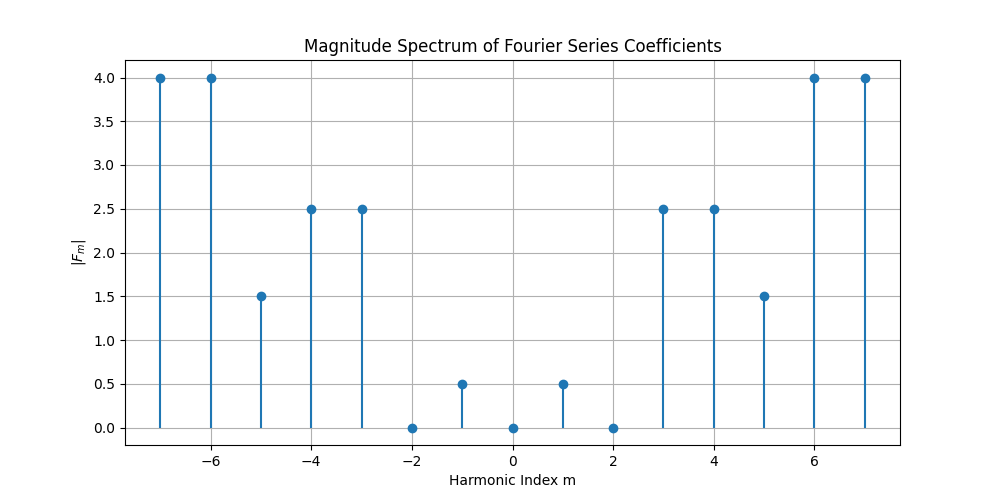
\includegraphics[width=1\linewidth]{fourierseriescoefficients.png}
    \caption{Plot of Fourier Coefficients \(F_m\) as a sequence of m}
    \label{fig:placeholder}
\end{figure}
\begin{table}[H]
    \centering
    \begin{tabular}{ccc}
        Harmonic \(m\) & Fourier Coefficient \(|F_m|\) \\
        \hline
        \(\pm 1\) & 0.5 \\
        \(\pm 2\) & 0 \\
        \(\pm 3\) & 2.5 \\
        \(\pm 4\) & 2.5 \\
        \(\pm 5\) & 1.5 \\
        \(\pm 6\) & 4 \\
        \(\pm 7\) & 4 \\
    \end{tabular}
    \caption{List of Fourier Coefficients \(F_m\)}
    \label{tab:placeholder}
\end{table}

The corresponding physical frequencies \(\omega_m\) occur at \(\omega_m = \frac{2\pi m}{T}\). They are as follows:
\begin{table}[H]
    \centering
    \begin{tabular}{ccc}
        Harmonic \(m\) & Physical Frequency \(\omega_m\) \\
        \hline
        \(\pm 1\) & \(\frac{2\pi}{T}\) \\
        \(\pm 2\) & \(\frac{4\pi}{T}\) \\
        \(\pm 3\) & \(\frac{6\pi}{T}\) \\
        \(\pm 4\) & \(\frac{8\pi}{T}\) \\
        \(\pm 5\) & \(\frac{10\pi}{T}\) \\
        \(\pm 6\) & \(\frac{12\pi}{T}\) \\
        \(\pm 7\) & \(\frac{14\pi}{T}\) \\
    \end{tabular}
    \caption{List of Fourier Coefficients \(F_m\)}
    \label{tab:placeholder}
\end{table}



\section{Time Function and Sampling}
Given:
\[
f(t) = \sum_{m=1}^{7} a_m \sin(\frac{2m\pi t}{T})
\]
where \(a_m\) is:
\[
[1, 0, 5, 5, 3, 8, 8]
\]
and \(T=1\), we have the plot of one full period of the time function \(f(t)\):
\begin{figure}[H]
    \centering
    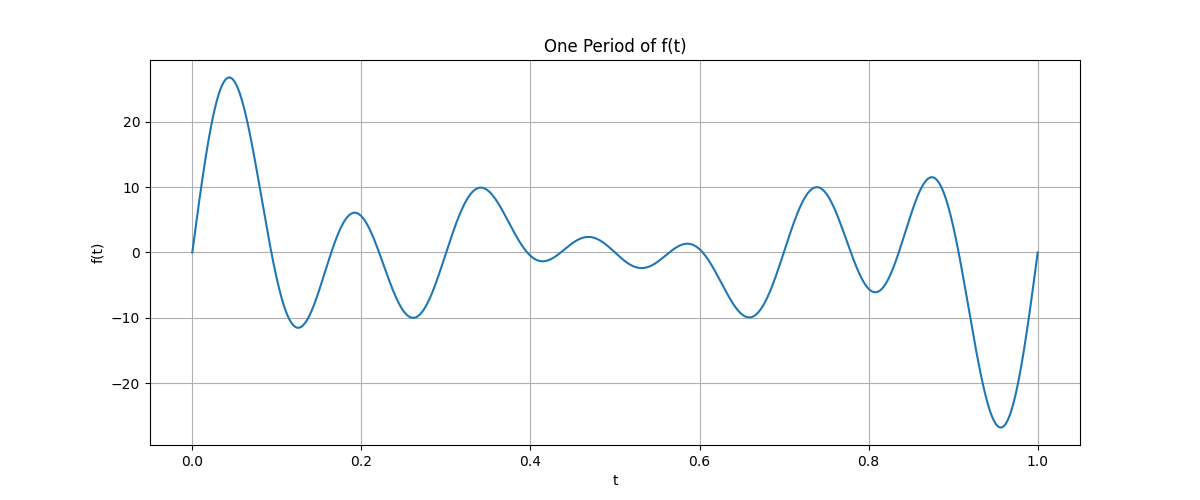
\includegraphics[width=1\linewidth]{oneperiodft.png}
    \caption{One full period of the time function \(f(t)\), from \(t=0\) to \(t=T\)}
    \label{fig:placeholder}
\end{figure}

Sampling \(f(t)\) at \(t=n\Delta t\), where \(\Delta t = \frac{T}{32}\), we have 32-point sample sequence:
\[
f[n] = \sum_{m=1}^{7} a_m \sin(\frac{2\pi m}{32} n)
\]
\begin{figure}[H]
    \centering
    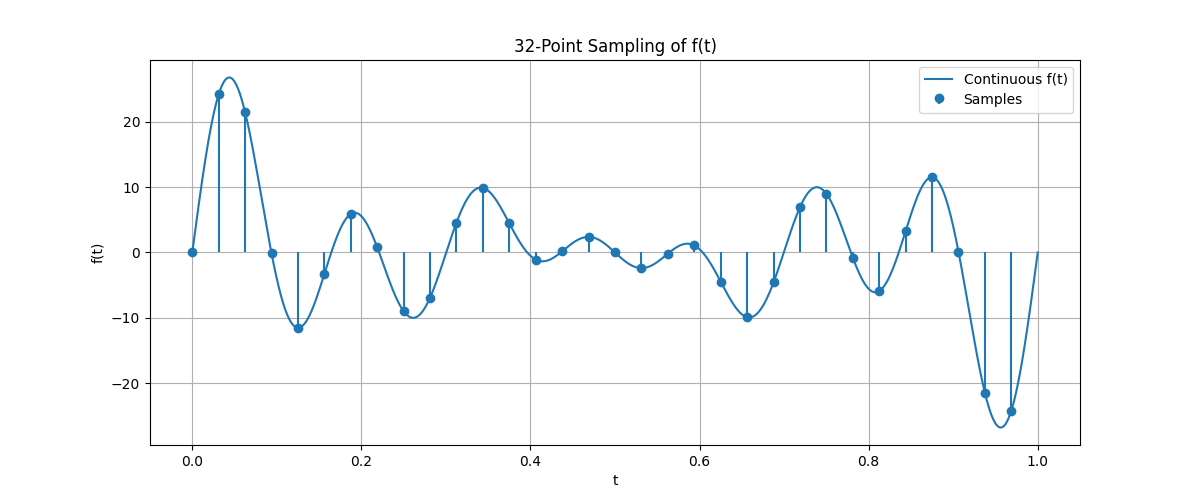
\includegraphics[width=1\linewidth]{32pointsampleft.png}
    \caption{The 32-point sample sequence \(f[n]\)}
    \label{fig:placeholder}
\end{figure}

\section{Fourier Transform of Periodic Functions}
Given:
\[
f(t) = \sum_{m=1}^{7} a_m \sin(\frac{2m\pi t}{T})
 = \sum_{m=1}^{7} \frac{a_m}{2j} (e^{j2\pi  \frac{mt}{T}} - e^{-j2\pi  \frac{mt}{T}})
\]
and:
\[
\mathcal{F} \{e^{j\omega_0 t} \} = 2\pi \delta(\omega - \omega_0)
\]
The Fourier Transform \(F(j\omega)\) of the periodic function \(f(t)\) is:
\[
F(j\omega) = \sum_{1}^{7} \frac{a_m\pi}{j} [\delta(\omega - m\frac{2\pi}{T}) - \delta(\omega + m\frac{2\pi}{T})]
\]

\begin{figure}[H]
    \centering
    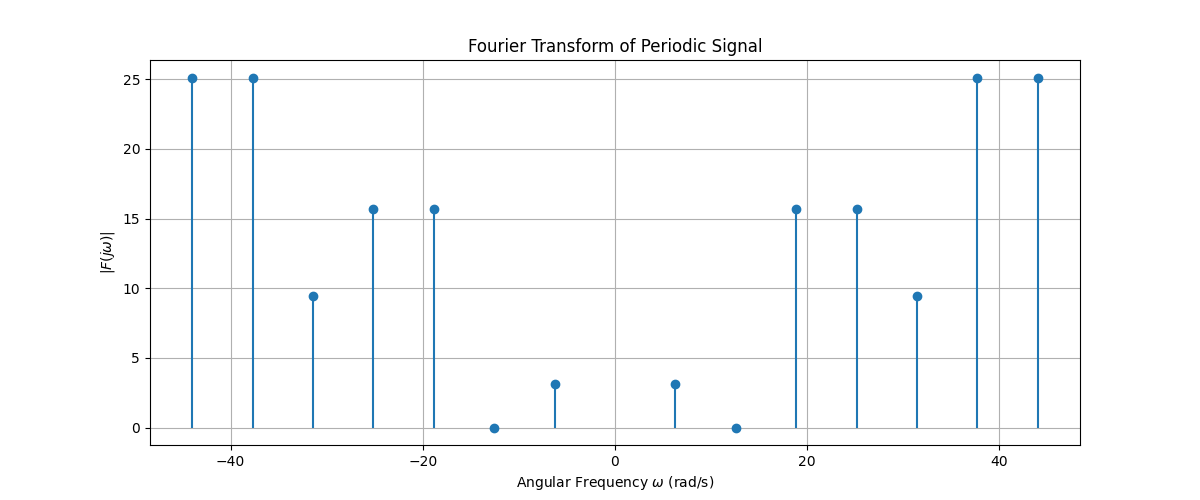
\includegraphics[width=1\linewidth]{fouriertransformperiodicsignal.png}
    \caption{Fourier Transform \(F(j\omega)\) of \(f(t)\)}
    \label{fig:placeholder}
\end{figure}

The spectrum contains impulses at \(\omega = \pm m\omega_0\) for \(m= 1, 2, 3, 4, 5, 6, 7\).
\begin{table}[H]
    \centering
    \begin{tabular}{ccc}
        Harmonic & Peak Location & Amplitude \\
        \hline
        1 & \(\pm \omega_0\) & \(\pi\) \\
        2 & \(\pm 2\omega_0\) & \(0\) \\
        3 & \(\pm 3\omega_0\) & \(5\pi\) \\
        4 & \(\pm 4\omega_0\) & \(5\pi\) \\
        5 & \(\pm 5\omega_0\) & \(3\pi\) \\
        6 & \(\pm 6\omega_0\) & \(8\pi\) \\
        7 & \(\pm 7\omega_0\) & \(8\pi\) \\
    \end{tabular}
    \caption{Amplitudes and physical frequencies of the peaks}
    \label{tab:placeholder}
\end{table}

\section{DTFT}
For the 32-point sampled sequence \(f[n] = f(n\Delta t)\) with \(\Delta t = \frac{T}{32}\), the discrete-time signal becomes:
\[
f[n] = \sum_{m=1}^{7} a_m \sin(\frac{\pi m}{16}n)
\]
with peaks occurring at \(\Omega_m = \pm m\frac{\pi }{16}\) for \(m = 1, 2, 3, 4, 5, 6, 7\).
\begin{figure}[H]
    \centering
    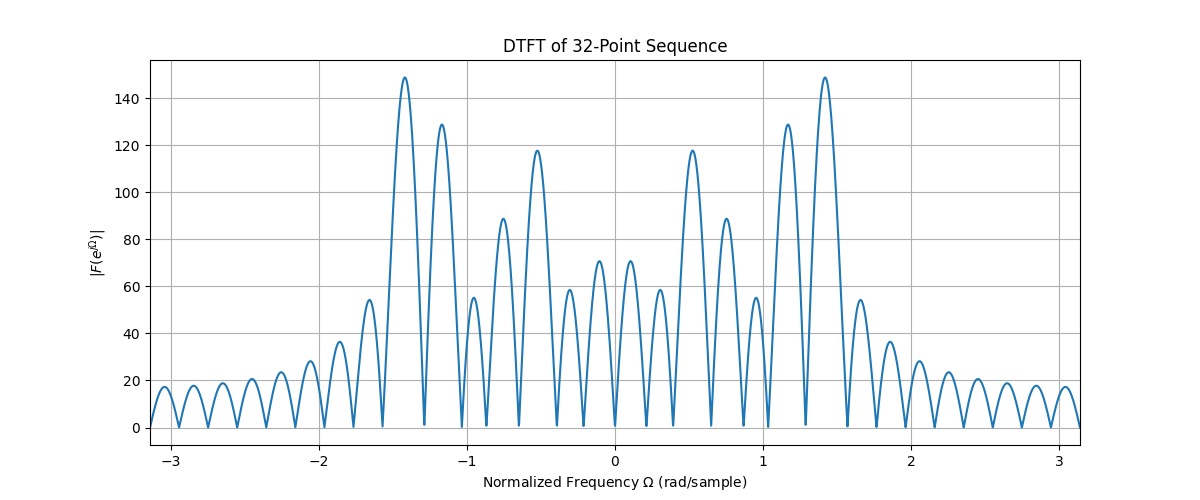
\includegraphics[width=1\linewidth]{dtft32pointsequence.png}
    \caption{The DTFT \(F(e^{j\theta})\) of the 32-point sequence \(f[n]\)}
    \label{fig:placeholder}
\end{figure}

The peaks will have an amplitude of approximately \(16a_m\) because we only have 32 samples.
\begin{table}[H]
    \centering
    \begin{tabular}{ccc}
        Harmonic & Peak Location & Amplitude \\
        \hline
        1 & \(\pm \frac{1\pi}{16}\) & 16 \\
        2 & \(\pm \frac{2\pi}{16}\) & 0 \\
        3 & \(\pm \frac{3\pi}{16}\) & 80 \\
        4 & \(\pm \frac{4\pi}{16}\) & 80 \\
        5 & \(\pm \frac{5\pi}{16}\) & 48 \\ 
        6 & \(\pm \frac{6\pi}{16}\) & 128 \\
        7 & \(\pm \frac{7\pi}{16}\) & 128 \\
    \end{tabular}
    \caption{Amplitude and location of peaks}
    \label{tab:placeholder}
\end{table}

\section{DFT}
The 32-point DFT of \(f[n]\) is:
\[
F(k) = \sum_{n=0}^{31} \sum_{m=1}^{7} a_m \sin(\frac{2\pi m}{32}n) \ e^{-j\frac{2\pi n}{32}k}
\]
\[
F(k) = \sum_{n=0}^{31} \sum_{m=1}^{7} \frac{a_m}{2j} (e^{j\frac{2\pi m}{32}n} - e^{-j\frac{2\pi m}{32}n}) \ e^{-j\frac{2\pi n}{32}k}
\]
\[
F(k) = \sum_{n=0}^{31} \sum_{m=1}^{7} \frac{a_m}{2j} (e^{-j\frac{2\pi n}{32}(k-m)} - e^{-j\frac{2\pi n}{32}(k+m)}) 
\]
Peaks will occur at positive frequencies \(k = m\) and negative frequencies \(k = 32 -m\) for \(k = 1, 2, 3, 4, 5, 6 ,7\) with amplitude \(16a_m\).

\begin{figure}[H]
    \centering
    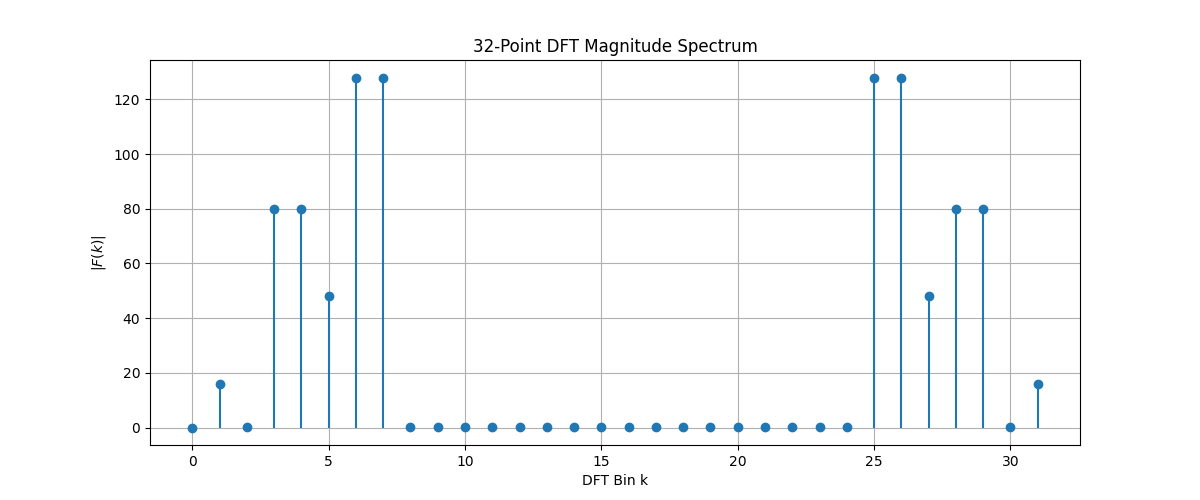
\includegraphics[width=1\linewidth]{32pointdftspectrum.png}
    \caption{32-point DFT spectral sequence \(F(k)\)}
    \label{fig:placeholder}
\end{figure}


\begin{table}[H]
    \centering
    \begin{tabular}{ccc}
        Harmonic & k & Amplitude \\
        \hline
        1 & 1, 31 & 16 \\
        2 & 2, 30 & 0 \\
        3 & 3, 29 & 80 \\
        4 & 4, 28 & 80 \\
        5 & 5, 27 & 48 \\
        6 & 6, 26 & 128 \\
        7 & 7, 25 & 128 \\
    \end{tabular}
    \caption{Amplitudes and locations of the peaks}
    \label{tab:placeholder}
\end{table}

\section{Spectral Analysis}
Given \(T\), the period of the original function, sampling spacing \(\Delta t = \frac{T}{32}\), and DFT length \(N=32\), we can formulate the correspondences to map the integer index \(k\) in the DFT spectrum \(F(k)\) back to the original physical frequency index \(\omega\) in \(F(j\omega)\). The DTFT frequency variable is frequency \(\Omega = \omega \Delta t\) and the DFT samples the DTFT at  \(\Omega = \frac{2\pi k}{N}\). We substitute and set the equations equal to each other:
\[
\omega\frac{T}{32} = \frac{2\pi k}{32}
\]
Therefore:
\[
\omega = \frac{2\pi k}{T}
\]
In the time domain, frequencies occurred at:
\[
\omega = \frac{2\pi m}{T}
\]
Thus, we have \(k = m\).
This means that the DFT bin index directly corresponds to the harmonic number of the continuous-time signal. 
To recover the original harmonic amplitude \(a_m\), divide the DFT peak magnitude by 16:
\[
a_m = \frac{|F(k)|}{16}
\] 

\end{document}
